\documentclass[12pt,notitlepage]{article}
\usepackage{fullpage}
\usepackage{hyperref}
\usepackage{graphicx}
\usepackage[margin=3em]{caption}

\begin{document}
\title{Looping Surveillance Cameras like in the Movies}
\author{Zach Banks \and Eric Van Albert}

\begin{titlepage}
    \begin{center}
    \vspace{3in}

    \noindent 
    \textsc{\Huge Looping~Surveillance~Cameras Like~in~the~Movies}

    \vspace{1em}

    \noindent
    \textit{\Large Live~modification of network streams without~interruption~of~service}

    \vspace{1.5in}

    \noindent
    {\large Zach~Banks \& Eric~Van~Albert}

    \vspace{1em}

    \noindent
    {\large \today}

    \end{center}

\vfill

\begin{abstract}
This project consists of the hardware and software necessary to hijack wired network communications. The hardware allows an attacker to splice into live network cabling without ever breaking the physical connection. This allows the traffic on the line to be passively tapped and examined. Once the attacker has gained enough knowledge about the data being sent, the device switches to an active tap topology, where data in both directions can be modified on the fly. Through our custom implementation of the network stack, we can accurately mimic the two devices across almost all OSI layers.

We have developed several applications for this technology. Most notable is the editing of live video streams to produce a ``camera~loop,'' that is, hijacking the feed from an Ethernet surveillance camera so that the same footage repeats over and over again. More advanced video transformations can be applied if necessary. This attack can be executed and activated with practically no interruption in service, and when deactivated, is completely transparent.
\end{abstract}
\end{titlepage}

\newpage

\section{Motivation}
This project was undertaken because it appears quite frequently in the movies, but is rarely depicted in a remotely reasonable manner. We set out to re-create it as true to the movies as possible to demonstrate exactly how practical it would be to create a camera loop.

\begin{figure}[h!]
    \centering
    %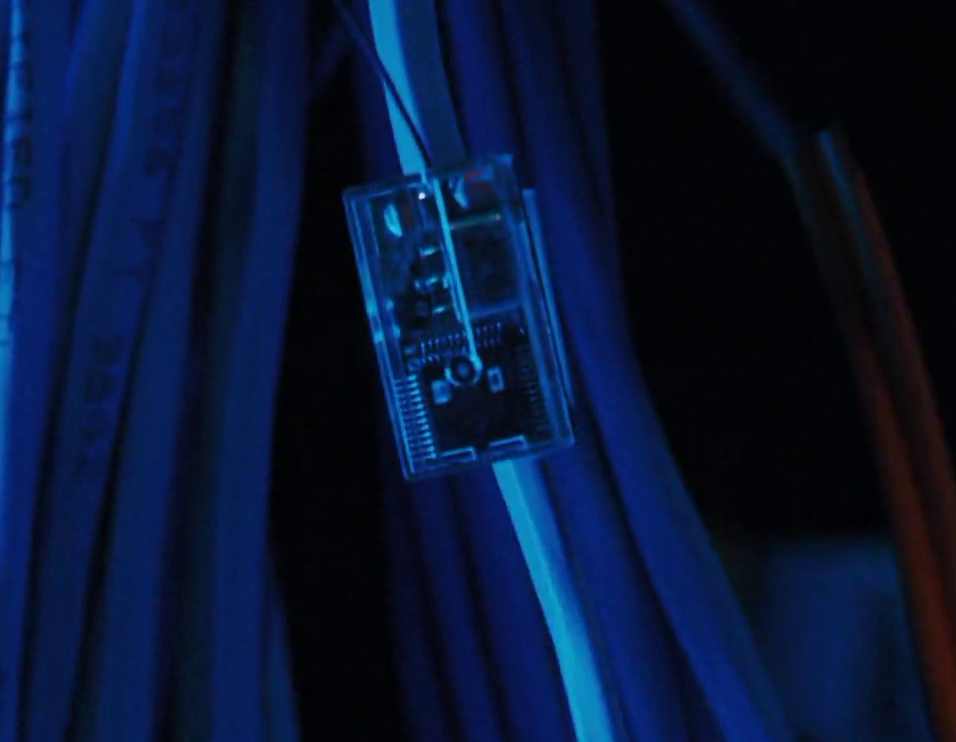
\includegraphics[width=0.45\textwidth]{oceanseleven}
    %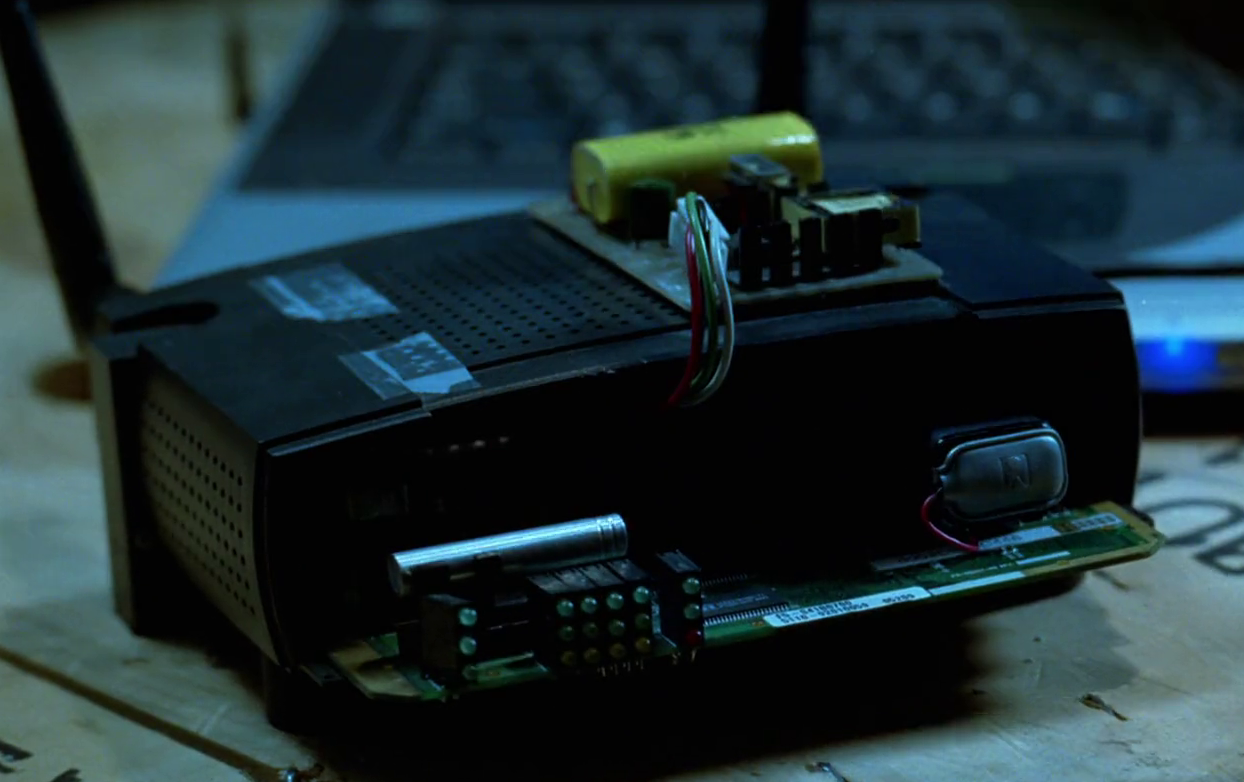
\includegraphics[width=0.45\textwidth]{nationaltreasure}
    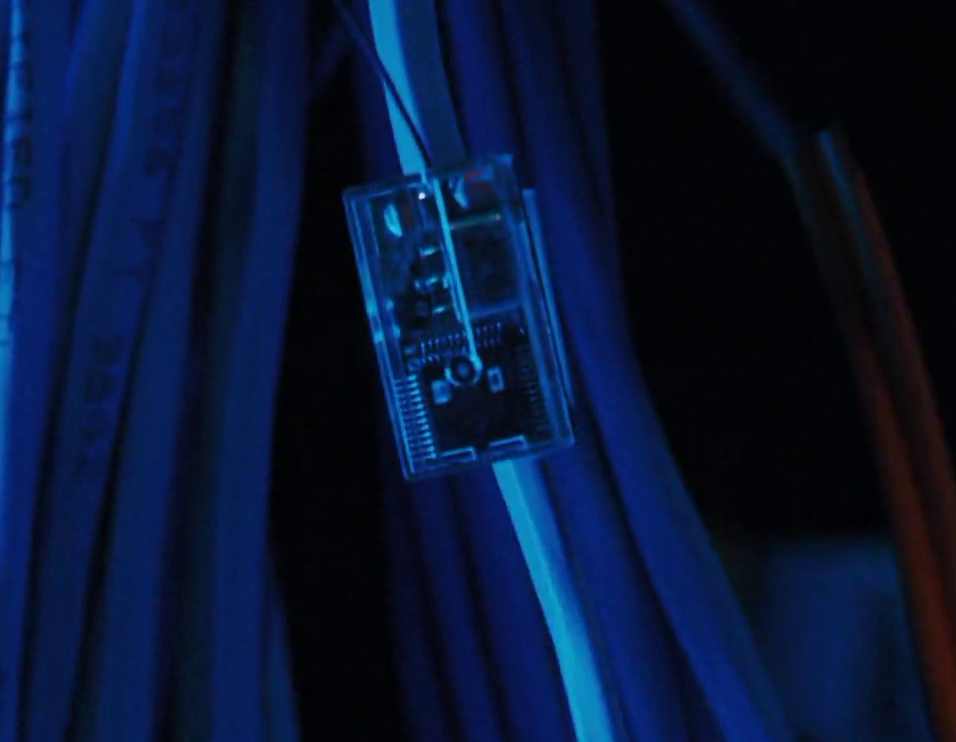
\includegraphics[height=2in]{oceanseleven}
    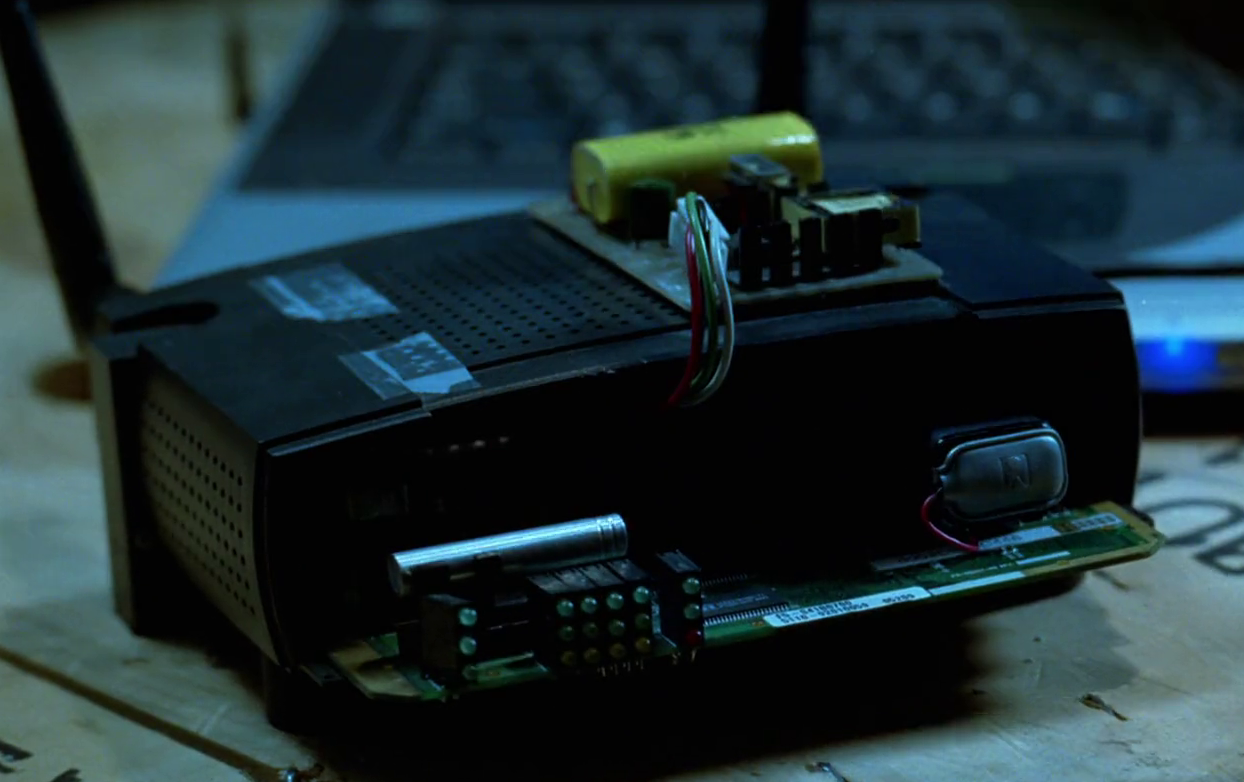
\includegraphics[height=2in]{nationaltreasure}
    \caption{Camera loop devices from \textit{Ocean’s Eleven} (2001, left) and \textit{National Treasure} (2004, right).}
\end{figure}

\section{Literature Review}

There has been a fair amount of previous work done on the topic of surveillance camera hacking.% 
\footnote{Black Hat 2013: \textit{Exploiting Network Surveillance Cameras Like a Hollywood Hacker} --- \url{https://www.youtube.com/watch?v=B8DjTcANBx0}}%
\footnote{DEFCON 17: \textit{Advancing Video Application Attacks with Video Interception, Recording, and Replay} --- \url{https://www.youtube.com/watch?v=QcsQ6UzMJiU}}
Because our attack requires physical access to the camera wire, it may seem less powerful than some existing attacks. However, accessing that wire may be more practical than adding a machine of your own to the network containing that camera.

We feel that our work is different in three main ways. First, it is more generic. It is not specific to a brand or model of camera. Because it works at the physical Ethernet level, it affects all Ethernet devices.

Second, our attack is more covert. We provide a hardware solution to gain access to the camera feed. This device is undetectable by software and may even be undetectable by network cable analyzers. Notably, it does not rely on any form of ARP spoofing or poisoning. The other attacks we have found involve making use of existing network access, which may show up in logs. These attacks can typically be defeated by simply keeping the surveillance cameras off of accessible networks or behind a firewall. Our attack works regardless of the network configuration and does not generate any ancillary network activity. 

Finally, our attack is more extensible than any existing attack. With the universal tap board, any physical layer that uses $100\Omega$ differential pairs can be tapped, as can any low-speed signal. Likewise, our \texttt{lens} network framework allows nearly transparent editing of many common network communication protocols such as HTTP, and RTP, and can be expanded to include many more.

\section{Hardware}

\begin{figure}[h]
    \centering
    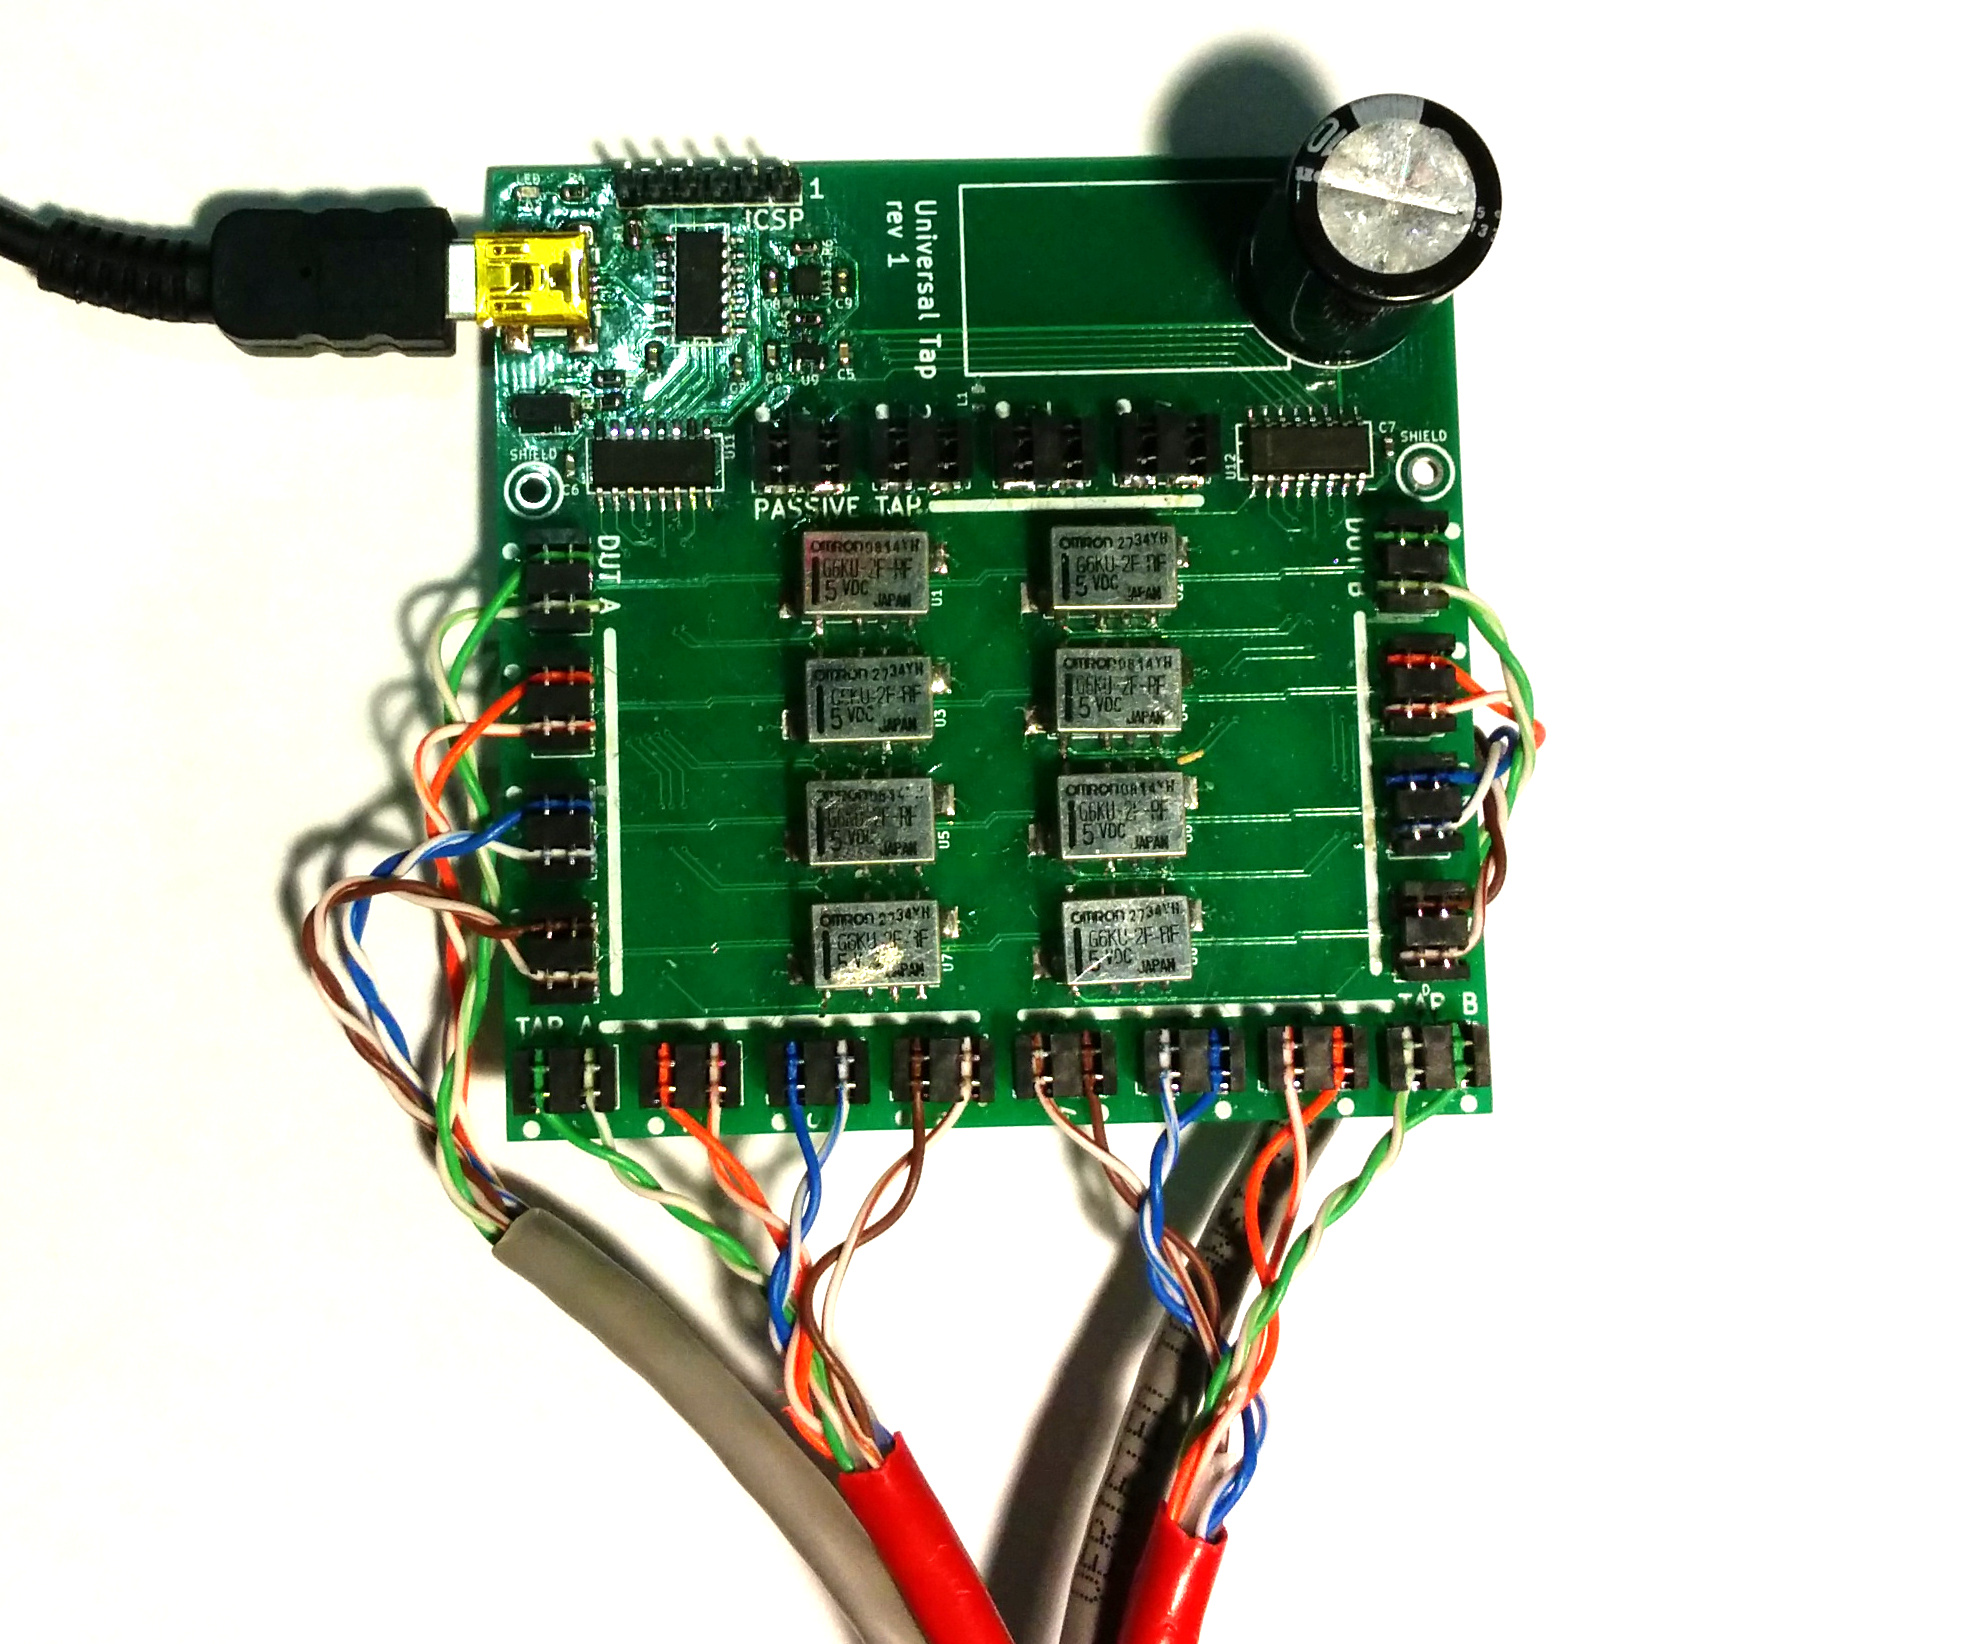
\includegraphics[width=0.45\textwidth]{hwphoto1}
    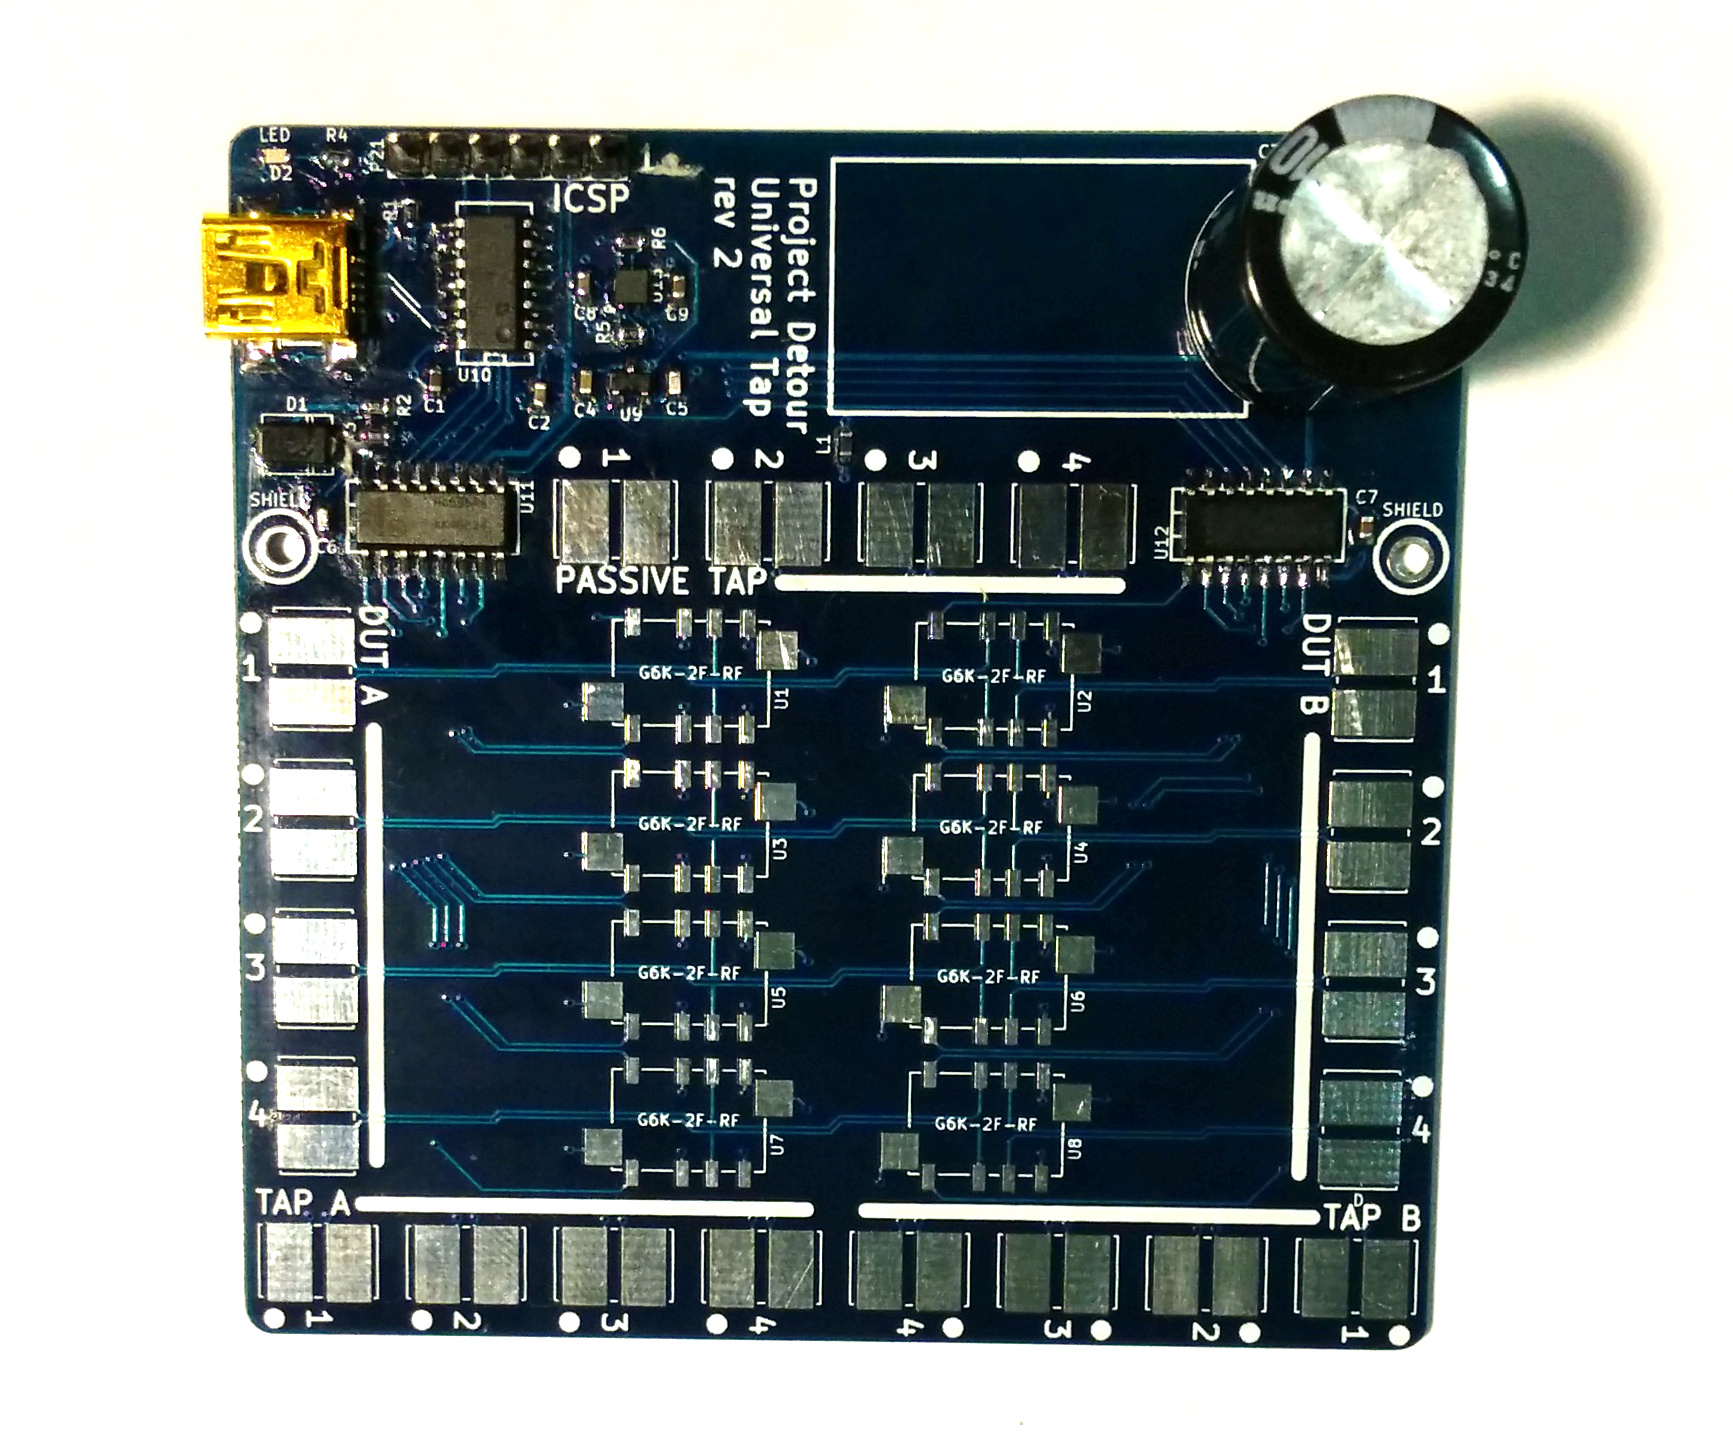
\includegraphics[width=0.45\textwidth]{hwphoto2}
    \caption{Two hardware revisions. On the left, an older version with cables spliced in. On the right, a new version in the process of being assembled}
\end{figure}

\newcommand{\textport}[1]{\texttt{#1}}

\begin{center}
    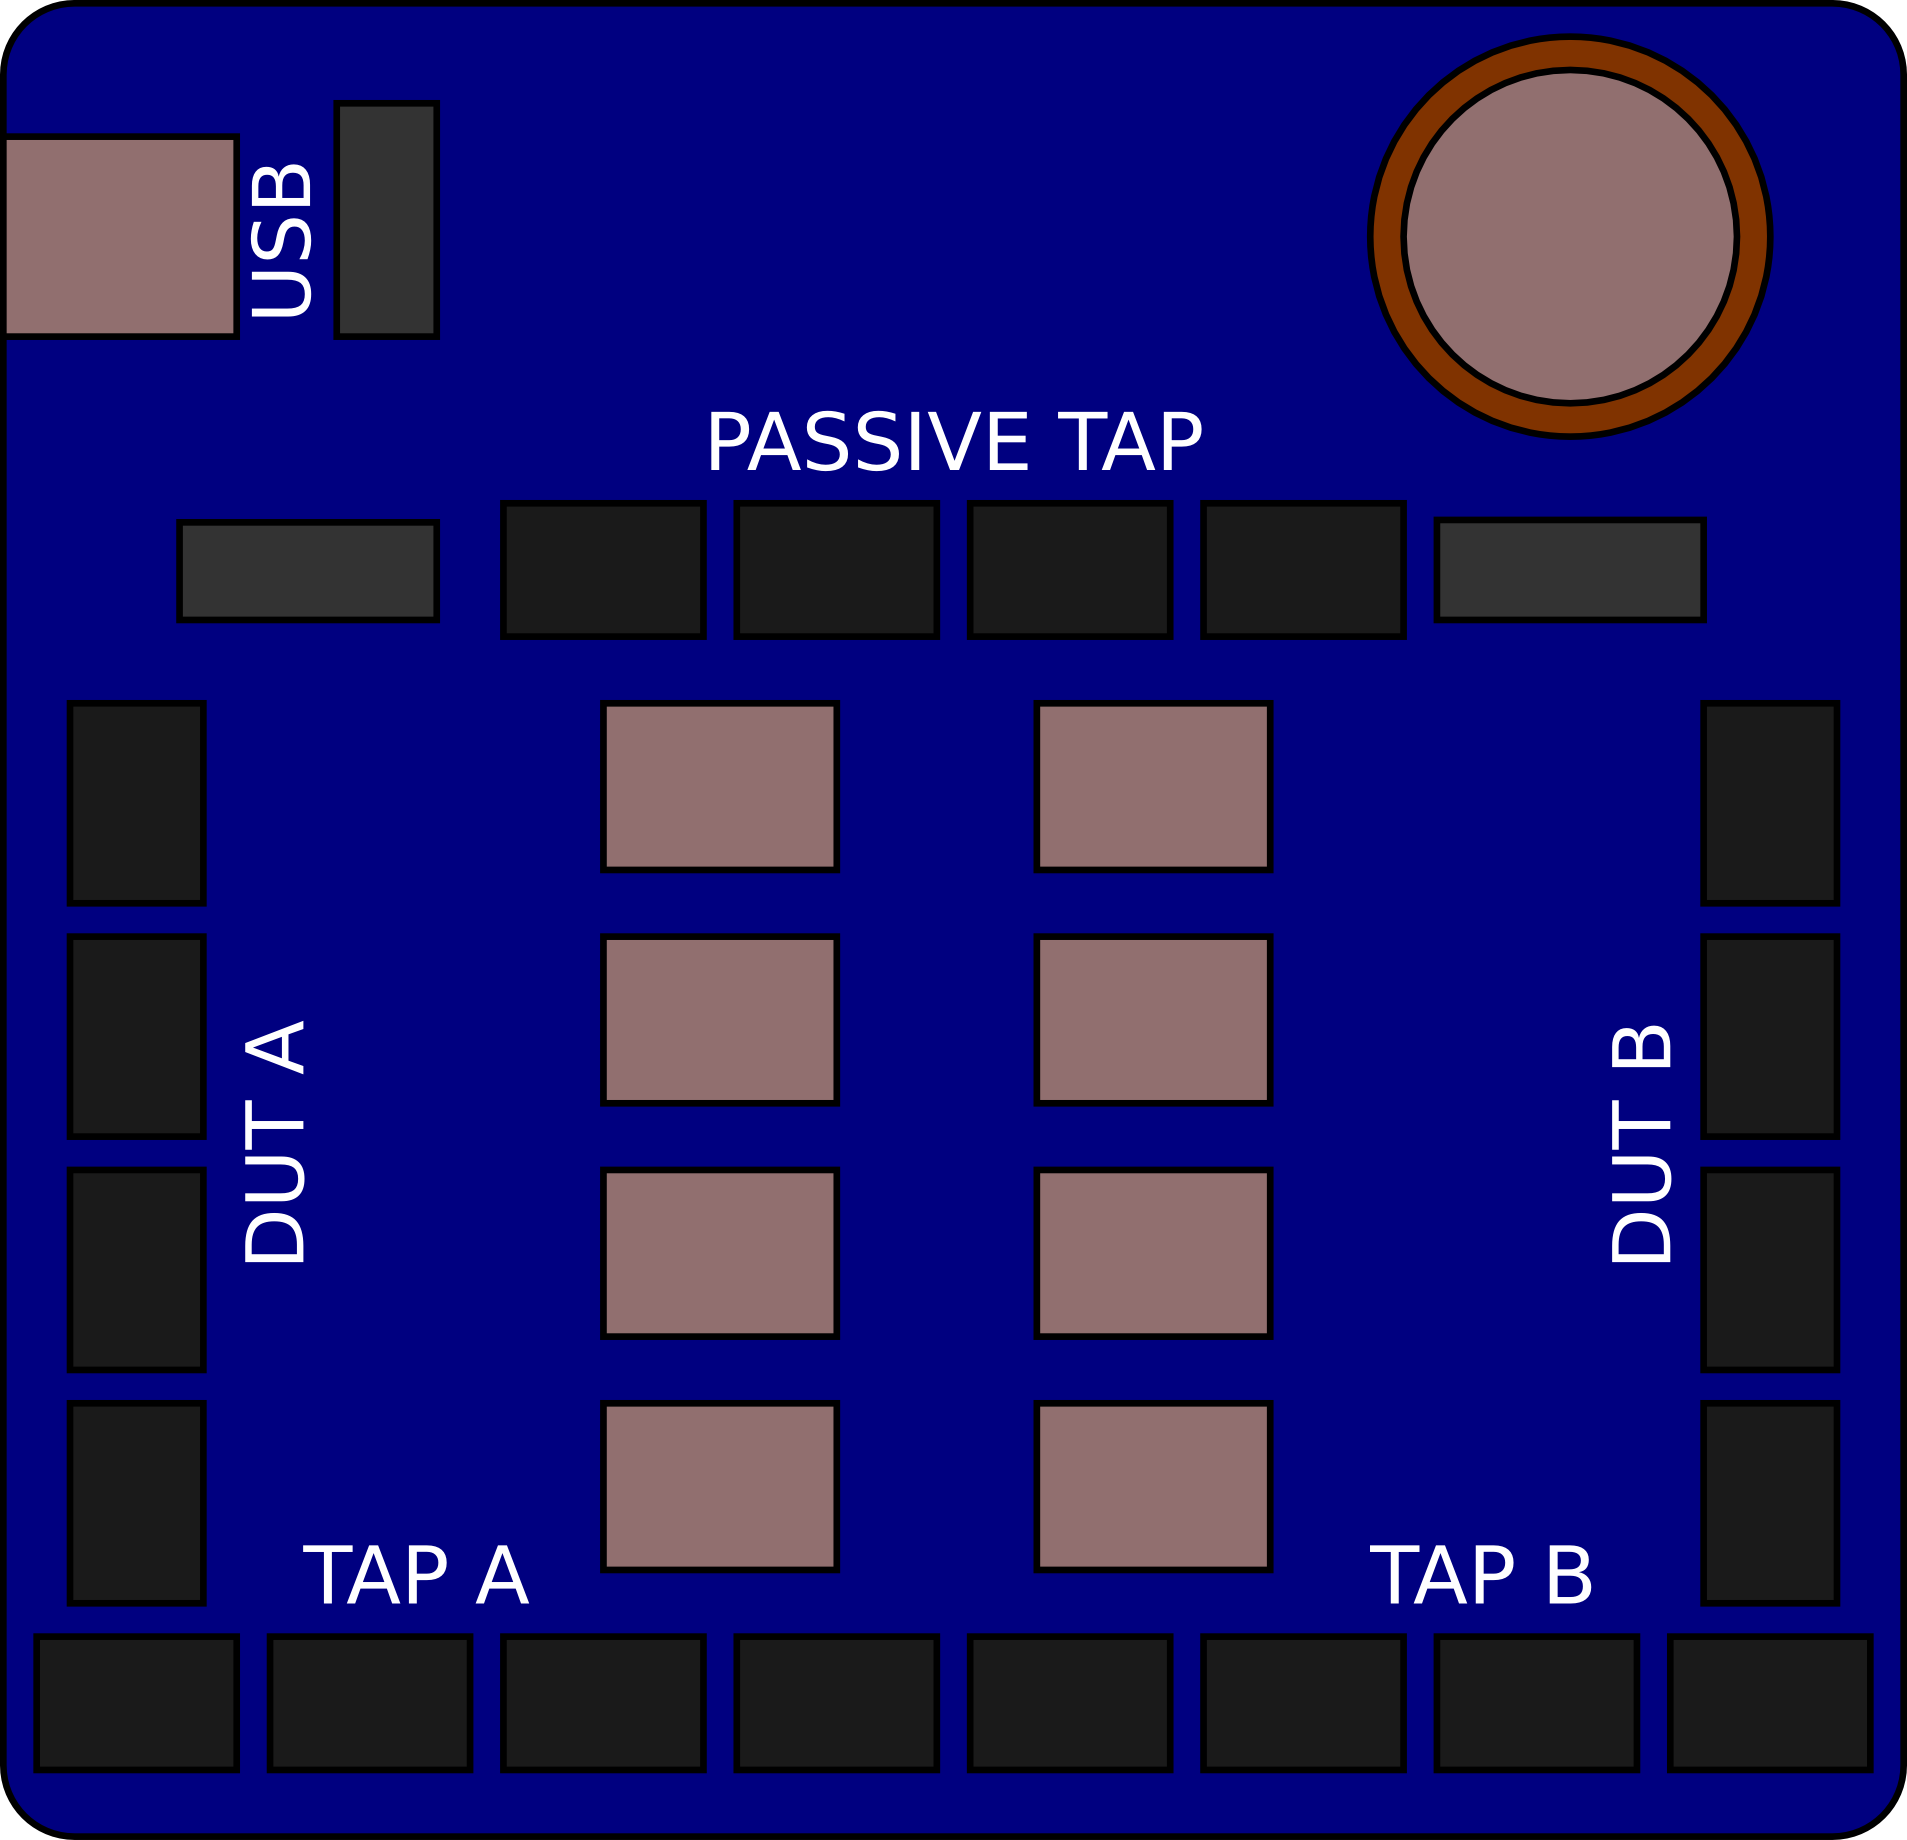
\includegraphics[width=0.6\textwidth]{detour_board}
\end{center}

The hardware consists of a custom PCB which acts as a USB-controlled universal tap. It has five ports, each of which is four differential pairs. The ports are designated \textport{DUT~A}, \textport{DUT~B}, \textport{TAP~A}, \textport{TAP~B}, and \textport{PASSIVE~TAP}. A set of high-bandwidth relays control the routing of these ports. By default, \textport{DUT~A} (\textit{Device~Under~Test~A}) passes directly through to \textport{DUT~B} and tees off to \textport{PASSIVE~TAP}.  Each port has punch-down connectors for wire insertion.

To insert the tap into a live cable, the line under test is spliced into both the \textport{DUT~A} and \textport{DUT~B} connectors. This adds a redundant copper path between the two devices. Passive monitoring is available on the \textport{PASSIVE TAP} port. Once the tap has been connected, the existing cabling can be cut so that all signals are now routed through just the tap board.

%TODO figures
\begin{center}
    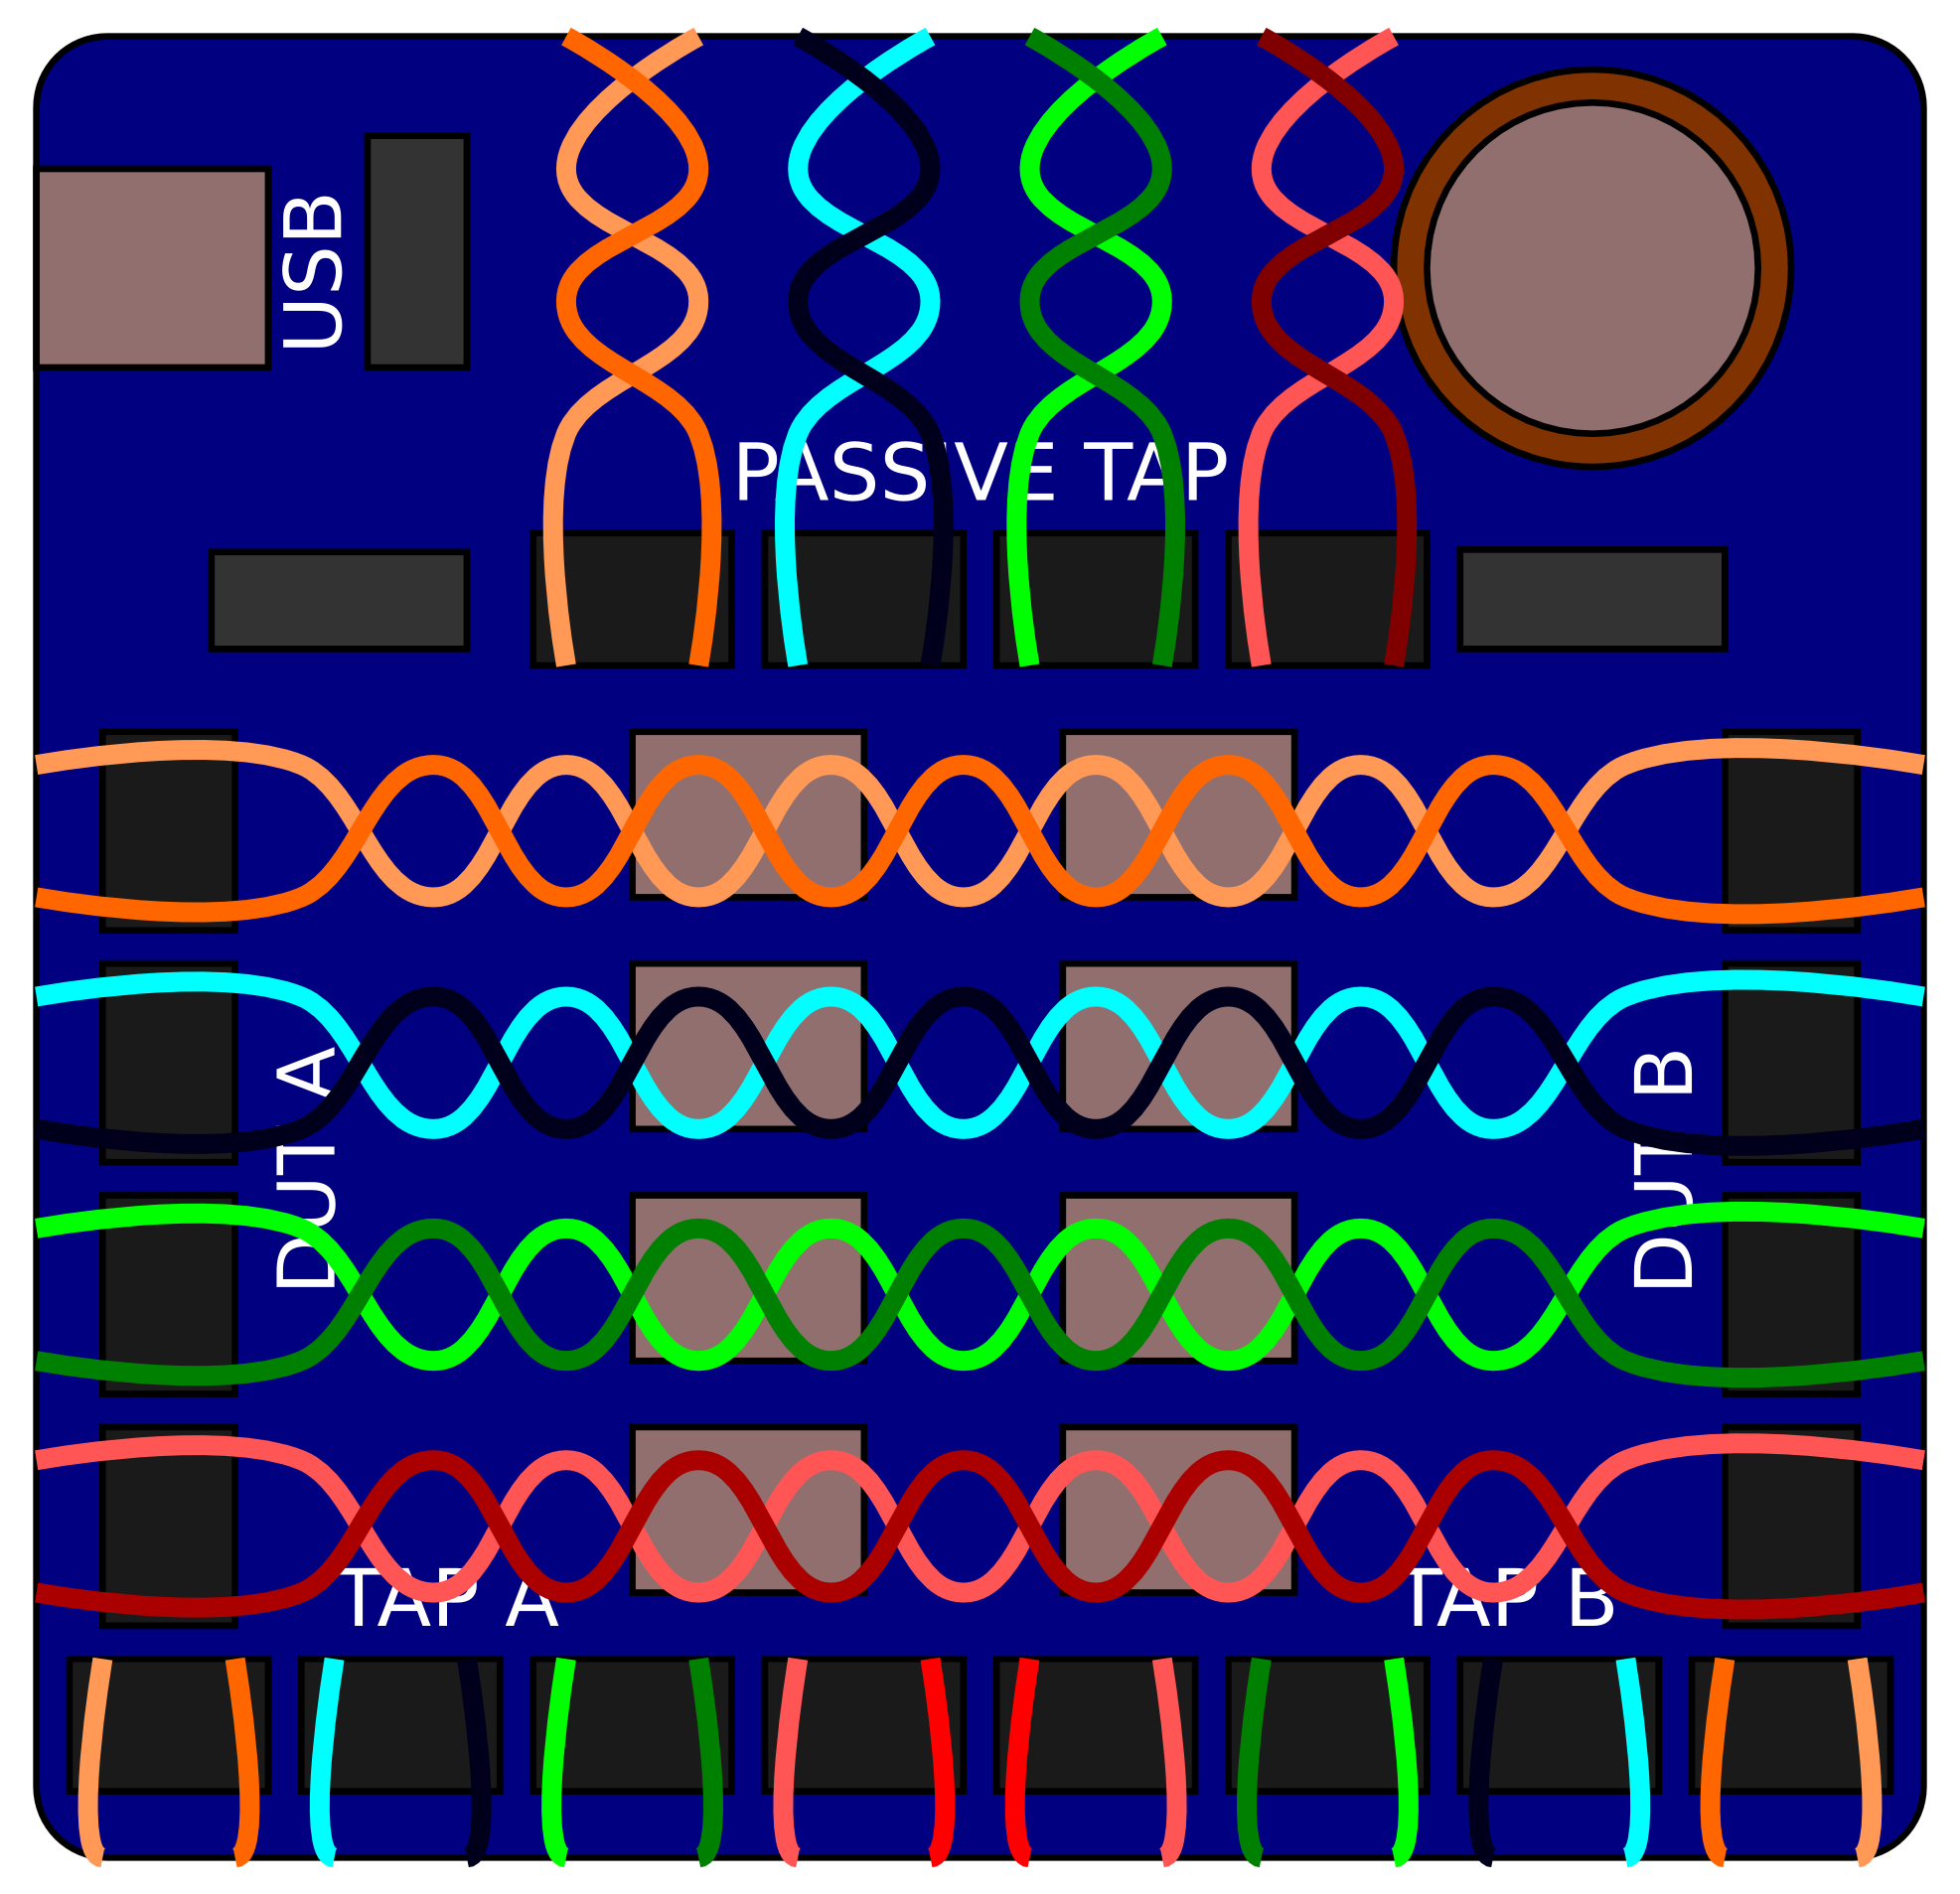
\includegraphics[width=0.45\textwidth]{detour_board_step_1}
    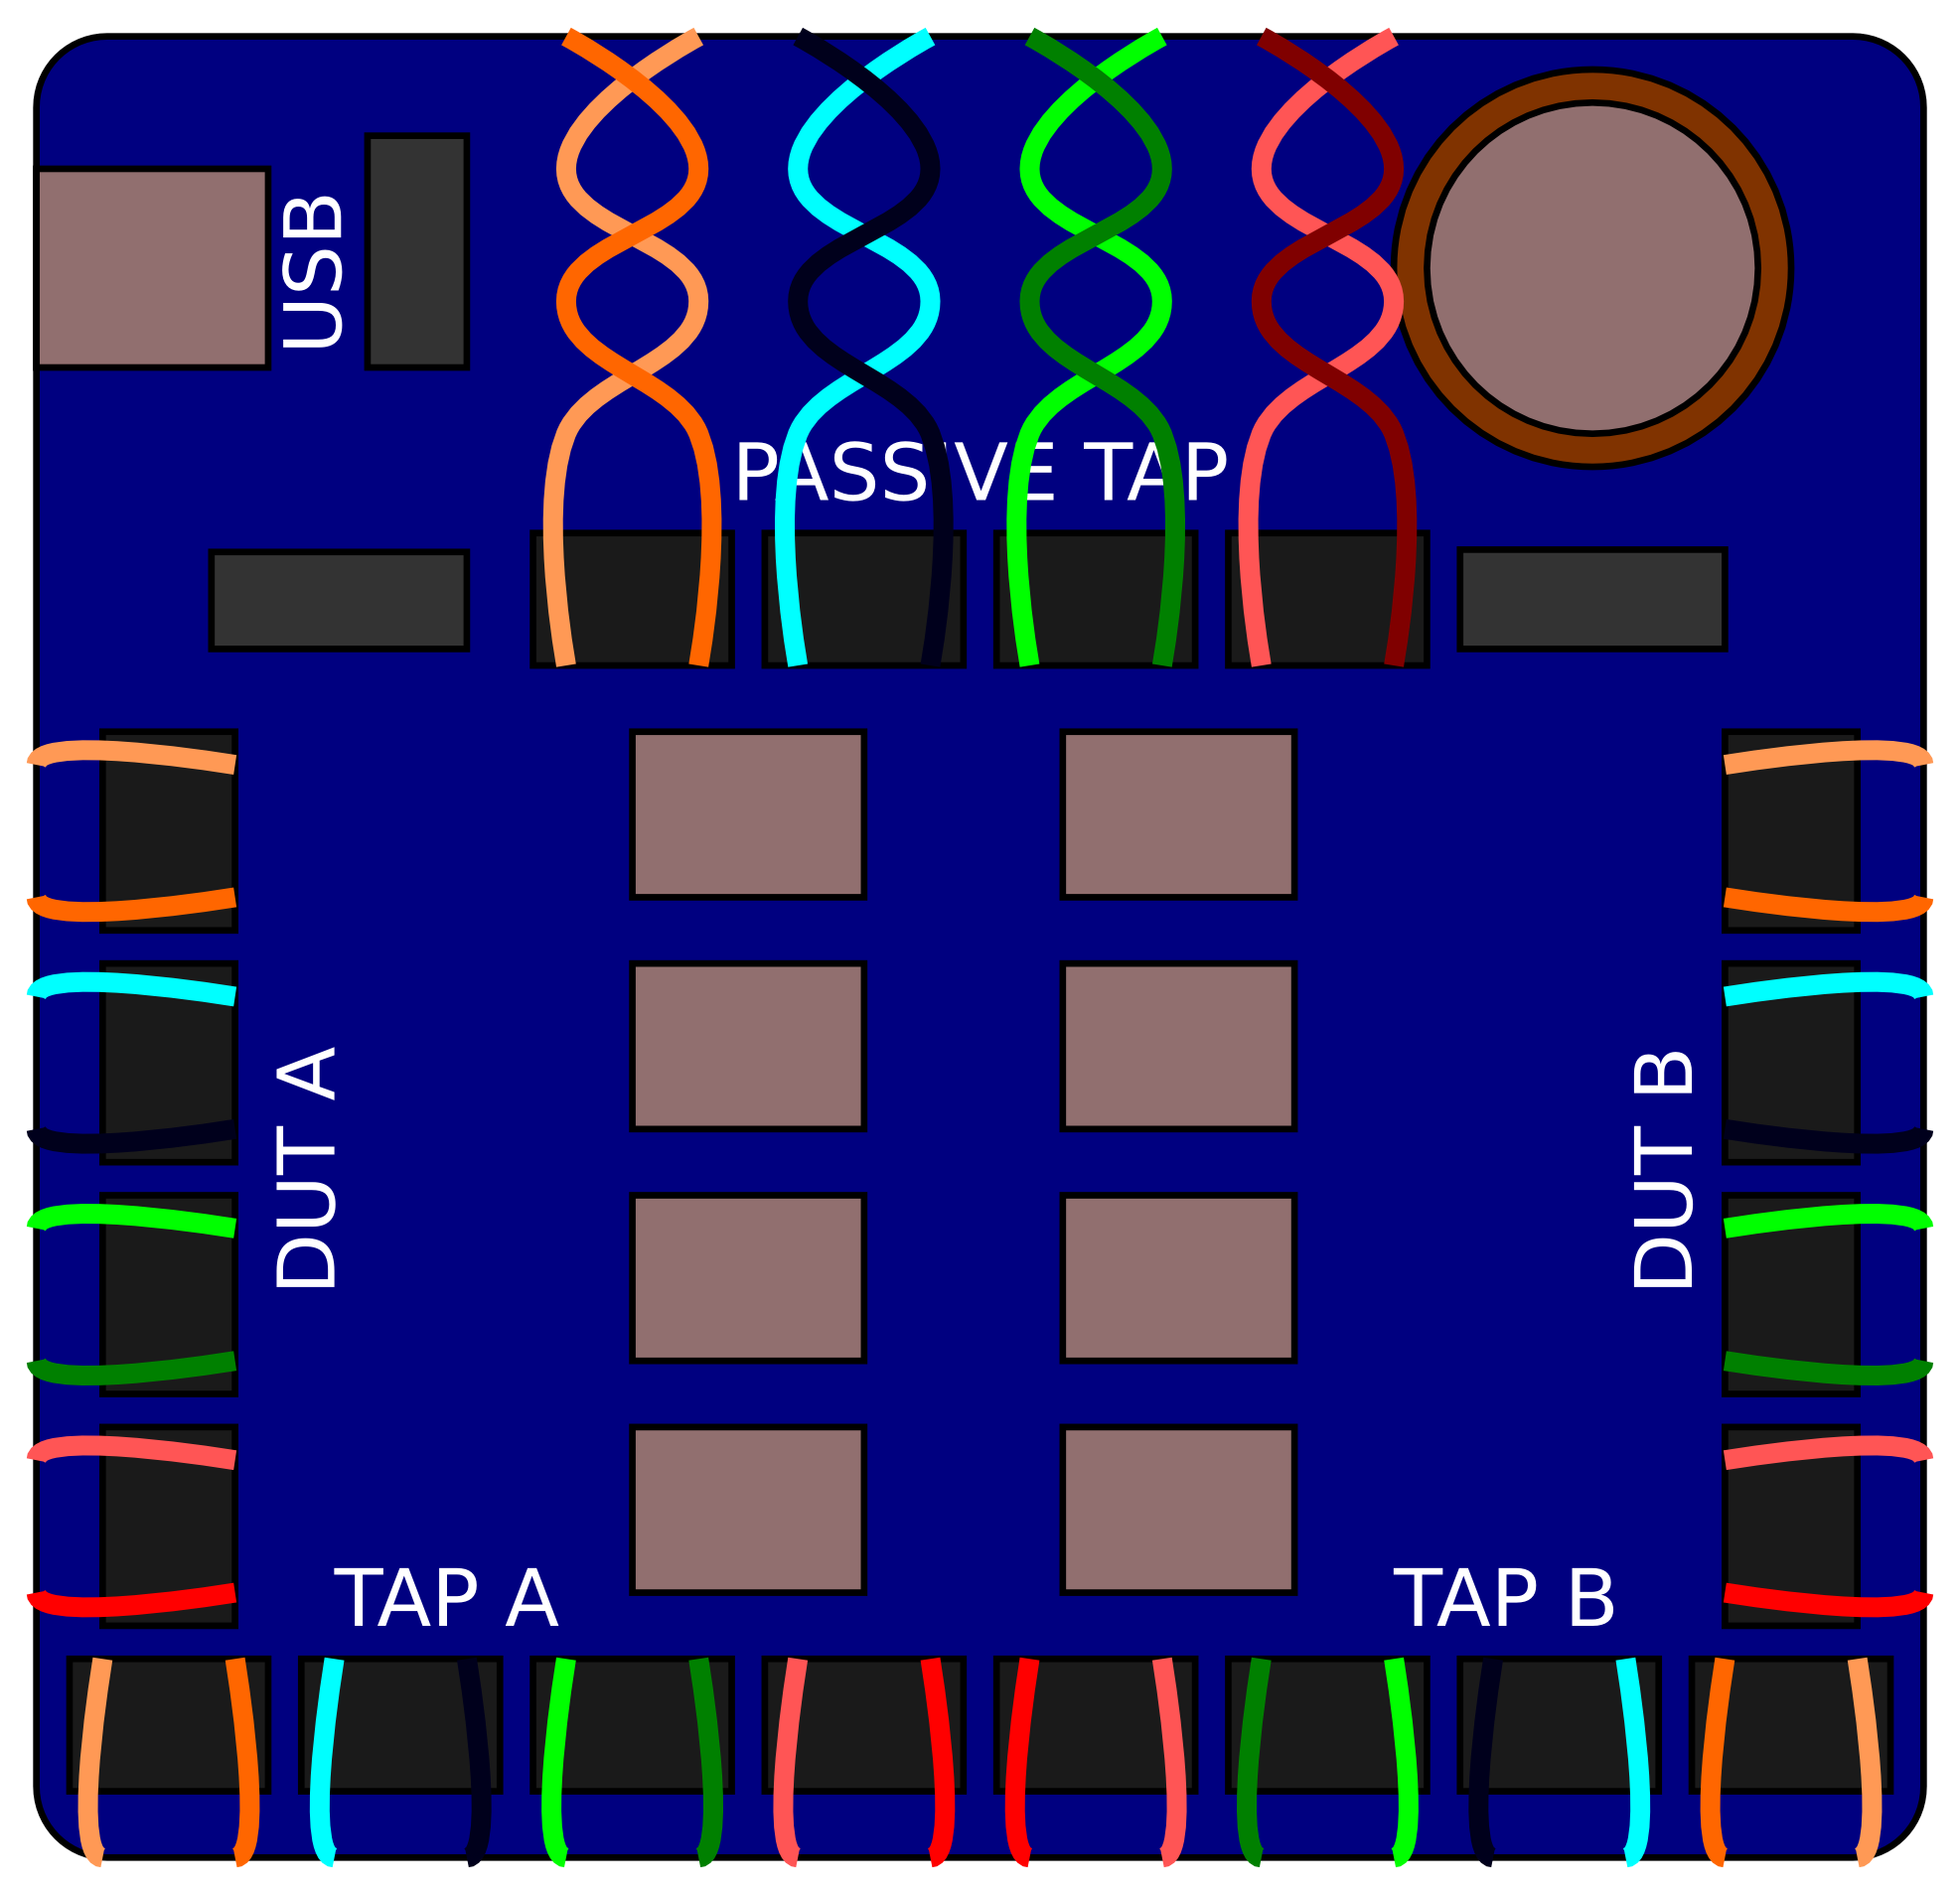
\includegraphics[width=0.45\textwidth]{detour_board_step_2}
\end{center}

The attacker then connects their man-in-the-middle device to the \textport{TAP~A} and \textport{TAP~B} ports. When commanded, the tap flips the relays to route \textport{DUT~A} to \textport{TAP~A}, and \textport{DUT~B} to \textport{TAP~B}. Traffic is now routed through the attacker's device in an active-tap configuration. The attacker is free to continue forwarding traffic transparently, or to generate fake traffic in either direction.

The tap board can be programmed to be fail-safe in the event of loss of USB communication or power. If a heartbeat signal from the host to device is lost, or power is disconnected, it can flip the relays back to transparent pass-through mode.

Finally, the tap board has a built-in accelerometer. It can use this in conjunction with a heartbeat signal from the device to the host to indicate tampering. If the board is unplugged or jostled from its resting position, the host will be alerted. The attacker can rest assured that the tap is in place, working, and undisturbed.

\section{Software}
Our software \texttt{lens} (\textit{Live~Editing~of Network~Streams}) aims to be as transparent and indetectable as possible while still enabling the attacker to capture, filter, modify, or spoof any packet. Although capturing packets is trivial, modifying or forging packets becomes increasingly difficult in higher OSI layers. To accomplish this, \texttt{lens} uses a custom network stack which allows the attacker to construct packets that are as similar as possible to those sent by the target devices. Additionally, \texttt{lens} is able to modify packets of stateful protocols (such as TCP) without interrupting the existing connection.
    
\begin{figure}[h]
    \centering
    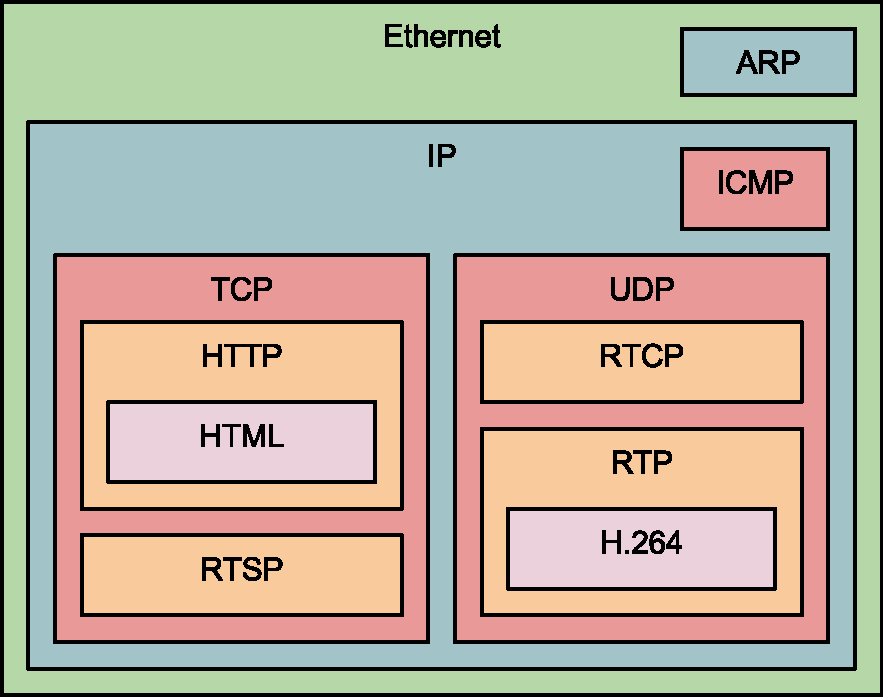
\includegraphics[width=0.5\textwidth]{osi_layers}
    \caption{The beefy 5-layer OSI burrito}
\end{figure}

    \texttt{lens} is implemented in Python (2.7) and is structured around tornado’s coroutine model. Each layer in the network stack is implemented separately and the layers are chained together in a pipeline-like fashion. Similar to the naitive network stack implemented by the operating system, each layer provides an abstraction to the next. For example, the TCP layer black-boxes the concept of open connections and their associated state for higher-up layers.

Starting with Ethernet, each layer decodes all packets that it recognizes. It examines the decoded data, and decides what to do. If it recognizes the protocol, it can pass it up the hierarchy for further decoding. If it doesn’t recognize the protocol, it does nothing. Most layers unwrap one protocol layer, but they could just also apply transformations to the data. Ultimately, a layer will re-encode the data back to its original protocol and pass it back down the hierarchy.

\begin{figure}[h]
    \centering
    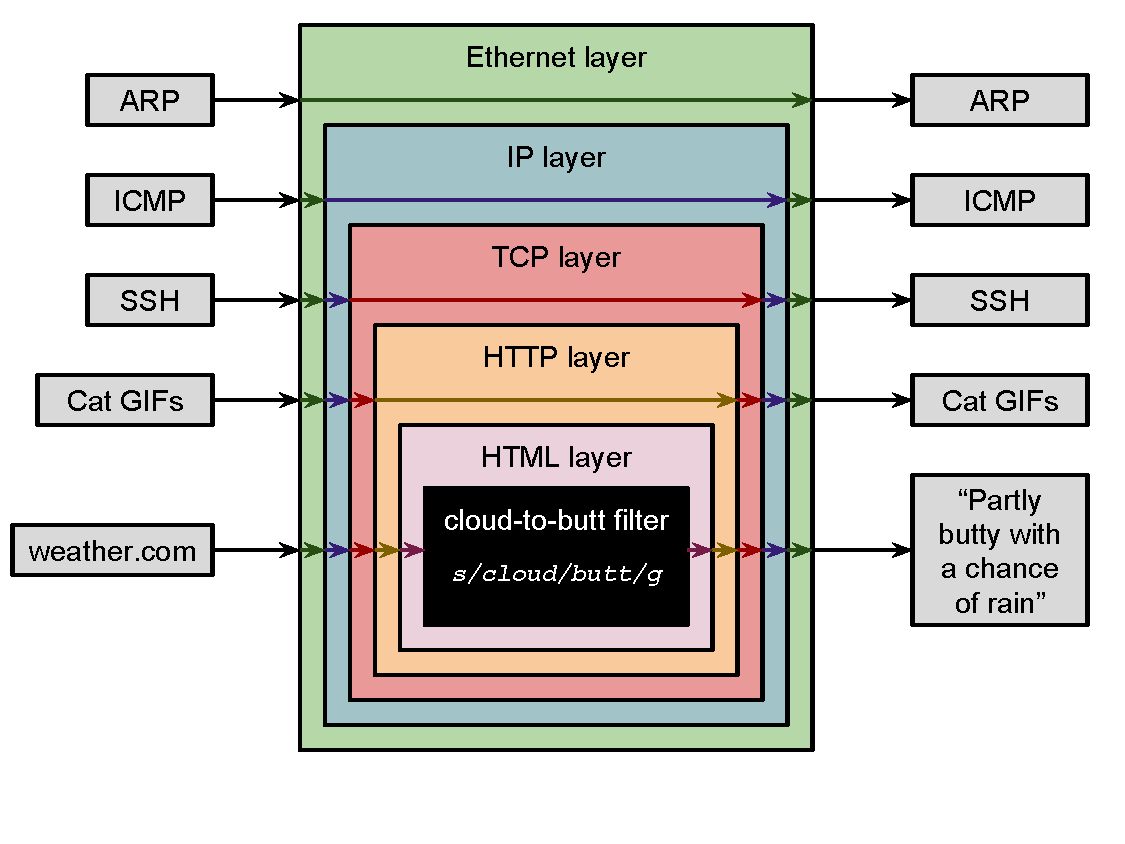
\includegraphics[width=0.5\textwidth]{lens_c2b}
    \caption{Graphical representation of \texttt{lens} mimicking the cloud-to-butt extension. Each arrow into a boundary indicates a software decoding or encoding step. A single simplex model is pictured here for clarity, however, \texttt{lens} can handle concurrent, duplex, and stateful transmissions.}
\end{figure}

Filter layers allow the attacker to perform transformations on given packets. For example, the infamous Cloud-to-Butt\footnote{\url{https://github.com/panicsteve/cloud-to-butt}} extension can be mimicked with a \texttt{lens} filter which performs a simple find-and-replace on the text at the HTTP layer.

To perform the camera loop, we use a more advanced set of filters. The camera sends its network stream over RTSP (Real Time Streaming Protocol), which uses TCP to set up the video stream, RTCP (RTP Control Protocol) over UDP for synchronization, and RTP (Real Time Protocol) over UDP to transport the H.264-encoded video. Each layer in \texttt{lens} parses apart incoming packets, applies any modifications, and reconstructs outgoing packets.

	In practice, video encoded with H.264 can be looped without re-encoding by concatenating the looped segment indefinitely. However, by re-encoding the stream with ffmpeg, an attacker can apply standard ffmpeg transformations to the video. For example, the attacker could loop most of the video, without modifying the corner of the frame that contains the timestamp.


\section{Further Work}
Using the \texttt{lens} framework and the universal tap board, an attacker can perform a camera loop attack on a networked camera without interrupting service. However, these tools can also be used to perform many other man-in-the-middle network attacks: such as TLS downgrade attacks or denial of service by packet filtering. 

	The universal tap board can also be used to tap cables other than Ethernet, such as HDMI. HDMI primarily sends data over four pairs of twisted differential pairs (1 clock, 3 data) which could be actively tapped with the universal tap board and modified with additional hardware. The tap board also supports simpler physical layers, such as USB~(1~twisted~pair) or Wiegand~(2~single-ended~lines). 

\end{document}
